\documentclass[12pt, letterpaper]{article}

\usepackage[utf8]{inputenc}
\usepackage{mathtools}
\usepackage{amsfonts}
\usepackage{amsmath}
\usepackage{graphicx}
\usepackage[a4paper, total={6in, 9in}]{geometry}

\DeclarePairedDelimiter{\ceil}{\lceil}{\rceil}

\title{CSE 21 HW 7}
\author{Brian Masse}
\date{March 5, 2025}

\begin{document}

\maketitle
\newpage

% MARK: Problem 1a

\bf{ 1. A slow-growing sequence of length n (with n \(\ge\) 1) is a non-decreasing sequence of integers that start with 1 and each pair of entries differ by at most 1. }

\-\ \newline
\-\ \it{ a) (for n \(\ge\) 1), How many slow-growing sequence of length n are there? }

\[A(n) = 2 \cdot A(n - 1), A(1) = 1\]
\begin{eqnarray*}
&1)& \textnormal{ } A(n) = 2 \cdot A(n - 1) \\
&2)& \textnormal{ } A(n) = 2^2 \cdot A(n - 1) \\
&\textnormal{  }& \vdots \\
&k)& \textnormal{ } A(n) = 2^k \cdot A(n - 1) \\
&\textnormal{  }& \vdots \\
&n - 1)& \textnormal{ } A(n) = 2^{n - 1} \\
\end{eqnarray*}

% MARK: 1b
\-\ \newline
\-\ \it{ b) How many bits would the most efficient fixed-length encoding of sequenes use? }


\begin{eqnarray*}
n &=& \ceil{ log_2( 2^{n - 1}) } \\
&=& n - 1
\end{eqnarray*}



% MARK: 1c
\-\ \newline
\-\ \it{ c) Develop your own encoding / decoding algorithm where the code uses this number of bits }

\-\ \newline
\textnormal{ Create an encoding such that each bit in the encoded binary string represents whether to add 1 or 0 to the previous number in the string. }


% MARK: 1d
\-\ \newline
\-\ \it{ d) Use your encoding to encode the follow slow-growing sequences }
\-\ \newline
\begin{itemize}
\item (1,2,3,3,3,4,4,5)
\textnormal{ = 1100101}

\item (1,1,1,2,2,3,4,4)
\textnormal{ = 0010110}

\item (1,2,2,3,3,4,5,6)
\textnormal{ = 1010111}
\end{itemize}

% MARK: 1e
\-\ \newline
\-\ \it{ e) Use your decoding to decode the following strings }
\begin{itemize} 
\item \textnormal{01010100}
\textnormal{ = (1,1,2,2,3,3,4,4,4)}
\item \textnormal{11100011}
\textnormal{ = (1,2,3,4,4,4,4,5,6) }
\item \textnormal{10111110}
\textnormal{ = (1,2,2,3,4,5,6,7,7) }
\end{itemize}


\newpage
\-\ \newline
% MARK: Problem 2a
\bf{ 2. Image files can be encoded using binary strings. In the most simple version, you can encode an \(n x m\) black and white image using \(nm\) bits with black corresponding to 0 and white corresopnding to 1. }
\-\ \newline
\-\ \newline
\bf{ We can use hexadecimal to encode each of the cunks of 4 pixels into a single hexadecimal character. }

\-\ \newline
\-\ \it{ a) How many bits are required to encode this image by encoding each pixel with 1 bit? }

\[nm = (96)(96) = 9216\]



% MARK: 2b
\-\ \newline
\-\ \it{ b) How many hexadecimal characters are needed for this image? }

\[ \left(\frac{96}{4}\right)(96) = 2304 \]

\begin{itemize}
\item \( \frac{96}{4} : \textnormal{Groups per row}\)
\item \( 96 : \textnormal{Number of Rows}\)
\end{itemize}


% MARK: 2c
\-\ \newline
\-\ \it{ c) Huffman encoding is actually used in image compression. What we cand o is compute the frequency table of the hexadecimal chracters and build a Huffman code based on that. Then encode the hexadecimal string using the Huffman code. Here is the frequncy table for this particular image:}

\-\ \newline
{
\centering
\begin{tabular}{ | l | l | l | l | l | l | l | l | l | l | l | l | l | l | l | l | r | }
    \hline			
    \textnormal{Character} & 0 & 1 & 2 & 3 & 4 & 5 & 6 & 7 & 8 & 9 & A & B & C & D & E & F \\
    \hline
    \textnormal{Weight} & 1113 & 104 & 63 & 67 & 77 & 49 & 54 & 73 & 103 & 39 & 32 & 70 & 47 & 82 & 83 & 248 \\
    \hline  
  \end{tabular}\par
}

\-\ \newline
\begin{itemize} 
\item Draw the huffman tree for the set of frequencies. \newline

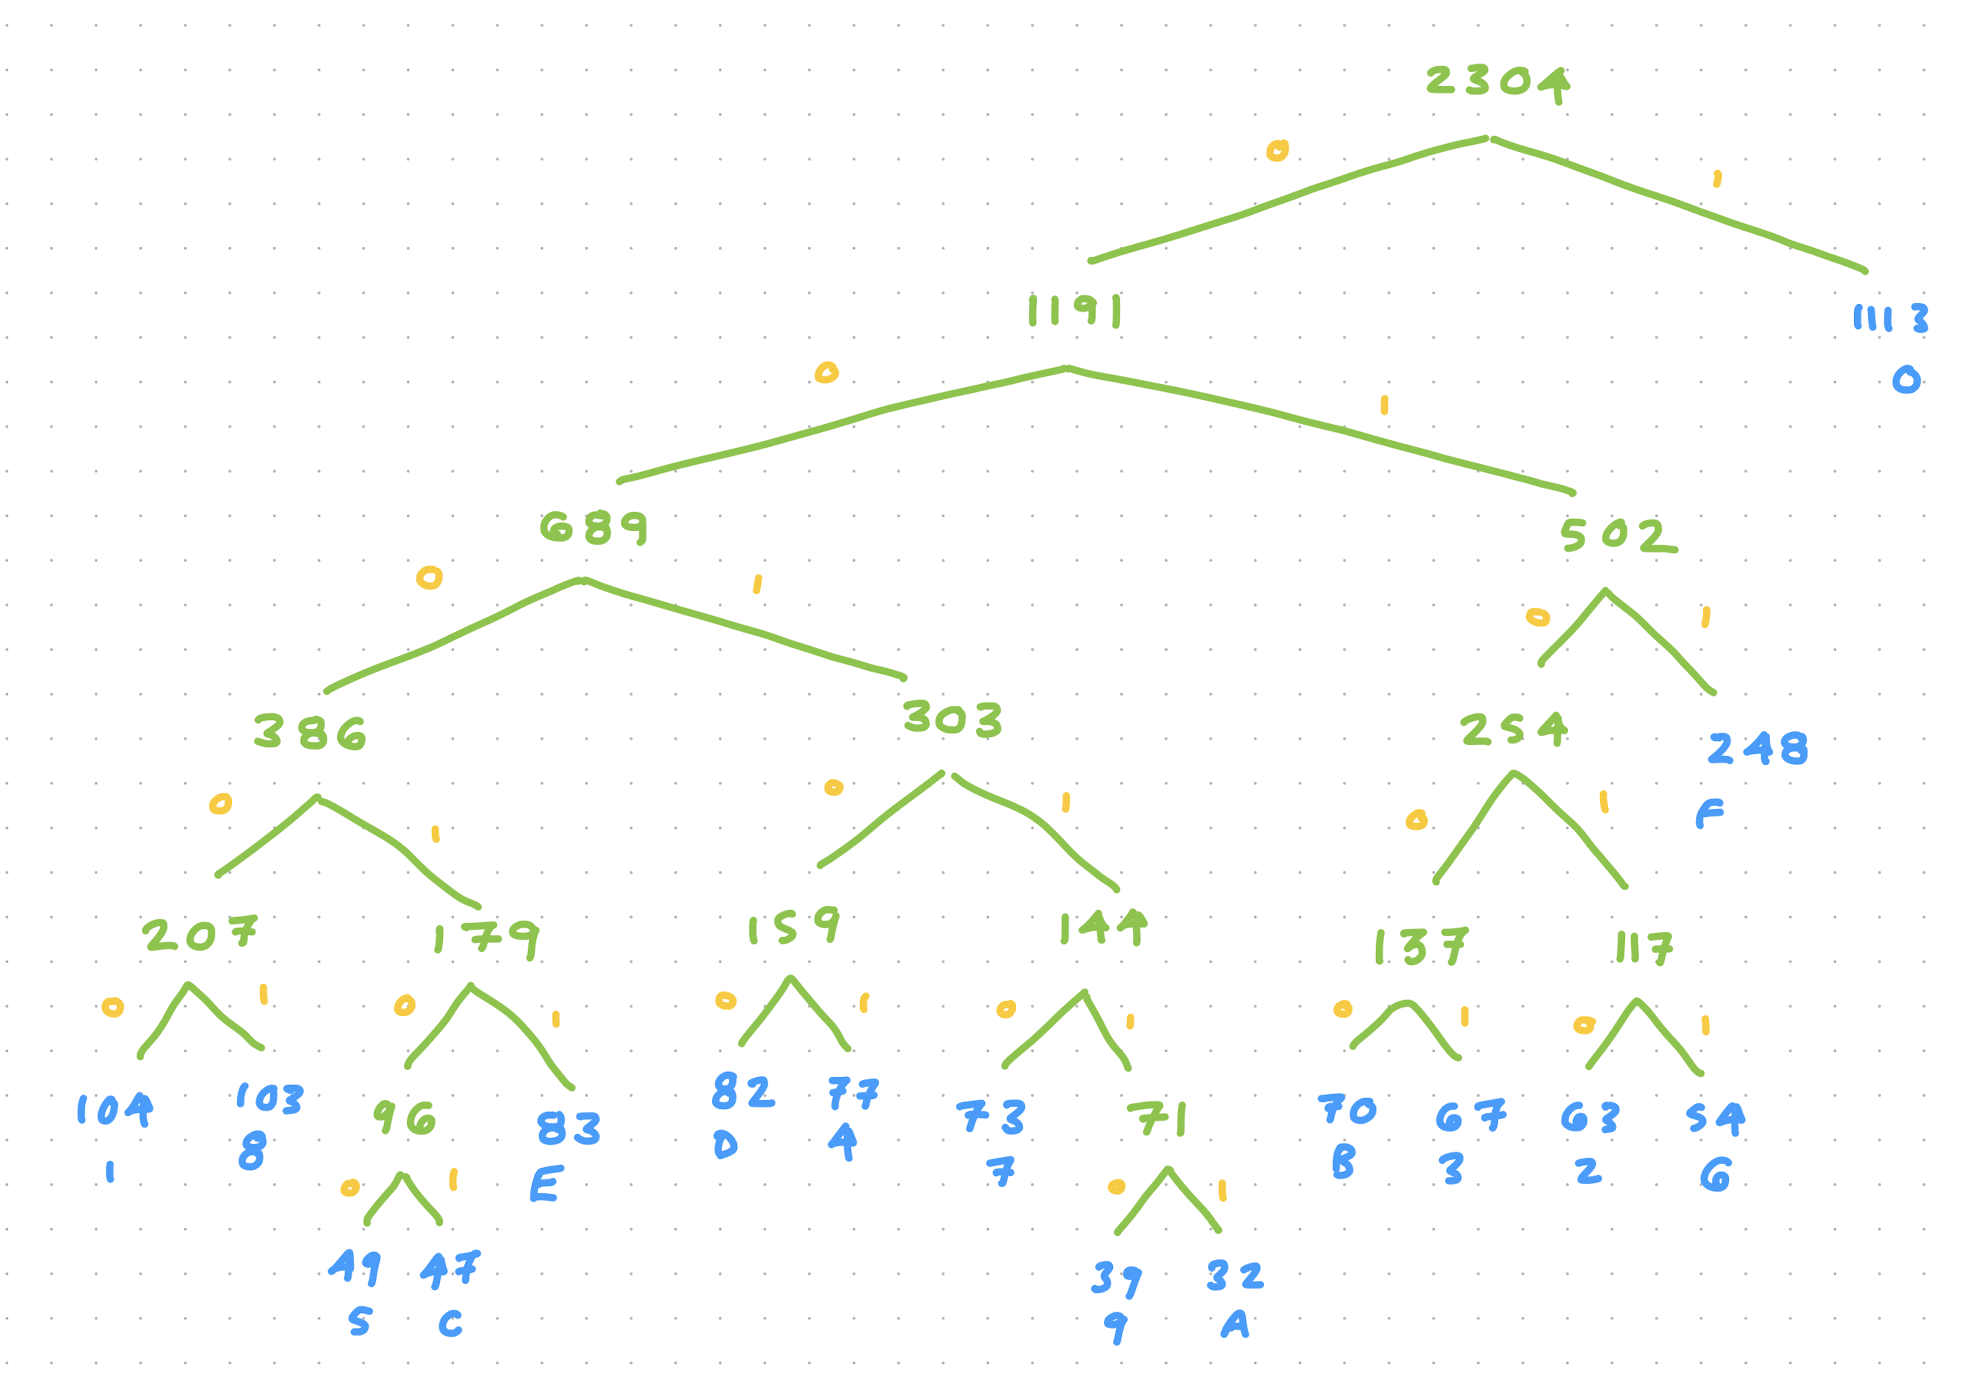
\includegraphics[width=0.85\textwidth]{graph1.png}

\item Give the code for each character

{
\centering
\begin{tabular}{ | l | l | r | }
    \hline			
    Number & Code \\
    \hline
    \textnormal{0} & \textnormal{1} \\
    \textnormal{1} & \textnormal{00000} \\
    \textnormal{2} & \textnormal{01010} \\
    \textnormal{3} & \textnormal{01001} \\
    \textnormal{4} & \textnormal{00101} \\
    \textnormal{5} & \textnormal{000100} \\
    \textnormal{6} & \textnormal{01011} \\
    \textnormal{7} & \textnormal{00110} \\
    \textnormal{8} & \textnormal{00001} \\
    \textnormal{9} & \textnormal{001110} \\
    \textnormal{A} & \textnormal{001111} \\
    \textnormal{B} & \textnormal{01000} \\
    \textnormal{C} & \textnormal{000101} \\
    \textnormal{D} & \textnormal{00100} \\
    \textnormal{E} & \textnormal{00011} \\
    \textnormal{F} & \textnormal{011} \\
    \hline  
  \end{tabular}\par
}

\-\ \newline
\item Calculate the total number of bits needed to encode this particular image of the moon using this coding.

\begin{eqnarray*}
T(n) = 1113(1) + 104(5) + 63(5) + 67(5) + 77(5) + 49(6) + 54(5) + 73(5) + 103(5) \\
+ 39(6) + 32(6) + 70(5) + 47(6) + 82(5) + 83(5) + 248(3)
\end{eqnarray*}

\end{itemize}


\newpage
% MARK: 3a
\-\ \newline
\bf{3. Consider the set of 26 capital letters of the Roman Alphabet}

\-\ \newline
\-\ \it{ a) Using a fixed length character-by-character encoding, what is the minimum number of bits required to encode each character? }

    \[ n = \ceil{ log_2(26) } = 5 \]

% MARK: 3b
\-\ \newline
\-\ \it{ b) Develop a fixed length character-by-character encoding for this alphabet using the number of bits from the previous part and use it to encode / decode the following strings }
\begin{itemize}
\item Encode: "MATH" 
\(\implies (13)(1)(20)(8) \implies\) 01101 00001 10100 01000

\item Encode: "BYTE" 
\( \implies (2)(25)(20)(5) \implies \) 00010 11001 10100 00101

\item Decode: 10010 01110 10001 10011
\( \implies (18)(14)(17)(19) \implies RNQS\)

\item Decode: 10001 01110 01110 10011 
\( \implies (17)(14)(14)(19) \implies QNNS\)
\end{itemize}

% MARK: 3c
\-\ \newline
\-\ \newline
\-\ \it{ c) Using fixed length encoding. What is the minimum number of bits required to encode each 4 letter string over this alphabet. }

\[ n = \ceil{ log_2{26^4} } = 19 \]

% MARK: 3d
\-\ \newline
\-\ \newline
\-\ \it{ d) Develop a fixed length encoding for 4 letter strings using the number of bits from the previous part and use it to encode / decode the following strings: }
\begin{itemize} 
\item Encode: "MATH"
\( \implies (13 \cdot 26^3 + 1 \cdot 26^2 + 20 \cdot 26 + 8) \implies 229692 \)

\( \implies \) 011 1000 0001 0011 1100 \newline


\item Encode: "BYTE"
\( \implies (2\cdot26^3 + 25\cdot 26^2 + 20\cdot 26 + 5) \implies 52577\)

\( \implies \) 000 1100 1101 0110 0001 \newline

\item Decode: 100 1111 1010 1001 0101
\( \implies 326293 \implies RNQS \)

\item Decode: 100 1011 0101 1001 1111
\( \implies 308639 \implies QNNS \)

\end{itemize}


\newpage
% MARK: Problem 4a
\bf{ 4. Suppose you are traveling from the bottom left corner of a 9 by 6 grid of city blocks and you wish to get to the top right corner only using up and right movements }

\-\ \newline
\-\ \it{ a) What is the minimum number of bits necessary to encode these paths with a fixed length encoding? }

\-\ \newline
\textnormal{There are \(6 + 9 \choose 6\) = \(15 \choose 6\) = \( 5005 \) number of paths from the bottom left to the top right, where 1s represent moving to the right.  }

\[ n = \ceil{ log_2{5005} } = 13 \]


% MARK: problem 4b
\-\ \newline
\-\ \it{ b) Develop an encoding strategy and encode the path given in the example }

\-\ \newline
\textnormal{Translate the path to a fixed-density binary string. Specifically, a length 13 binary strings with 6 1s, where 1 represents moving to the right and 0 represent moving up.}

\[ \textnormal{path} \implies 1 1110 0001 0001 00 \]

% MARK: problem 4c
\-\ \newline
\-\ \it{ c) Use your encoding strategy to decode the following string: 0 1010 1100 1100 }

\end{document}
